\chapter{Udviklingsmetoden}
\label{udviklingsmetoden}
I følgende kapitel vil vi beskrive og reflektere over den objektorienteret anlyse og design metode, som vi er blevet introduceret for i bogen Objektorientere Anlyse \& Design \cite{ooad}, samt over den evolutionære udviklingsmetode som vores projektforløb har taget udgangspunkt i. 

\section{Objektorienteret Analyse \& Design}
Objektorienteret Analyse \& Design er titlen på den bog, som vores tilgang og projektforløb har taget udgangspunkt i. Bogen beskriver en objektorienteret metode, til udvikling af systemer. Metoden består af fire hovedaktiviteter: Analyse af problemområde, Analyse af anvendelsesområde, Design af arkitektur og Design af komponenter \cite[p~ 15]{ooad}. Hvilke af aktiviteterne man udfører først, er ikke fast, men er helt op til det enkelte projektforløb. Vi modtog sideløbende med vores projekt, undervisning i kurset, hvor vi først blev introduceret for Analyse af problemområde, derefter Analyse af anvendelsesområde, Design af arkitektur og til sidst Design af komponenter. Derfor var det naturligt for os, også at følge denne rækkefølge, hvilket vi gjorde meget slavisk. Bogen præsenterer desuden en masse værktøjer, såsom rigebilleder, introduktion til prototyper mm. som er meget anvendelig i en udviklingsproces, hvor der er informanter/brugere involveret.

En af fordelene ved at anvende bogens objektorienteret analyse og design metode, er at programmeringen og implementeringen af systemet, bliver nemmere, da der efter analyse- og designdelen, ikke hersker nogen tvivl om, hvad systemet skal kunne, hvordan det er modelleret og hvordan det skal designes. Ulempen er at der skal bruges meget tid på at analysere og designe. I vores projektforløb, brugte vi endda ekstra lang tid, fordi vi først skulle sættes ind i, og forstå kursets begreber, før vi kunne anvende dem. Desuden var vi meget grundige med vores analyse- og designdel, og alle gruppens medlemmer deltog aktivt i eksempelvis, hvilke objekter, klasser og hændelser der var i problemområdet, hvordan klassernes tilstandsdiagrammer skulle se ud, hvilke aktøre vi skulle have osv. I det hele taget, brugte vi meget tid på at bearbejde og revidere diverse diagrammer. Tid, som vi kunne have brugt mere effektivt andet steds. Vi kunne eksempelvis have delt opgaverne ud, så alle ikke skulle side og kigge på det samme komponentdiagram, tilstandsdiagram osv. 

Til fremtidige projekter, vil vi anvende dele af den objektorienteret analyse og design metode, som kurset har introduceret. De mange gruppediskussioner vi i fællesskab har haft, har ledt os til en bedre forståelse for systemudvikling og de ting, feltet indebærer, og den objektorienteret metode vil formentligt kunne fungere endnu bedre, i et fremtidigt projekt, fordi vi nu har fået erfaring i at bruge den. Vi vurderer tilgengæld, at vi sandsynligvis ville kunne have lavet et ligeså godt produkt, med samme kvalitet, med mindre brug af den objektorienteret analyse \& design metode. Der blev brugt alt for meget tid på mindre detaljer, som hele gruppen brugte mange resurser på, som vi efterfølgende føler, ikke havde den store betydning, eller var trivielle og ville blive tilføjet eller redigeret naturligt undervejs, pga. den iterative udviklingsmetode, som vi beskriver i følgende \secref{sec:akadmiskevolutionaeremetode}.

%% Alle skulle være enige i det hele, og det tog endnu mere tid
%% Vi kan konkludere, at vi muligvis ville kunne have lavet et godt produkt á samme kvalitet på anden vis. 
%% Fordele og ulember ved metoden
%% Fremtidige projekter

\section{Den evolutionære udviklingsmetode}
\label{sec:akadmiskevolutionaeremetode}

Den evolutionære udviklingsmetode er velegnet i udviklingsprocesser af systemer og tager udgangspunkt i iterationer ved, at et forløb deles op i en række faser, som hver gennemgår samtlige af projektes dele. Et systemudviklingsprojekt kunne eksempelvis være delt op i følgende punkter: analyse, design, programmering, aftestning og afprøvning, som præsenteret i \figref{fig:evolutionaeremetode}. Figuren er, ligesom \figref{fig:konstruktivemetode}, taget fra slides, fra Objektorienteret Analyse \& Design \cite{ooadslide}, og tilpasset til vores eget projektforløb. Deres visuelle stil er genbrugt i \figref{fig:blandingsmetode}.

For hver fase vil der blive tilføjet, fjernet eller på anden vis redigeret i indholdet fra delene, så de hele tiden er opdateret i forhold til det problem, der skal løses. 
Metoden er specielt anvendelig i forhold til udviklingsprocesser, hvor det givne problem ikke er veldefineret, eller ændres undervejs i forløbet. 
I forhold til vores egen udviklingsprocess, havde vi i løbet af projektet havde vi specificeret et klassediagram, men det endelige klassediagram blev fastlagt i slutningen af projektforløbet, da vi først her var færdige med at fortolke og revidere vores forståelse af problemet.
Her kan udviklingsprocesen, ved hjælp af den evolutionære metode, nemt ændres og dirigeres henimod det rette problem igen.

\begin{figure}[ht]
	\centering
	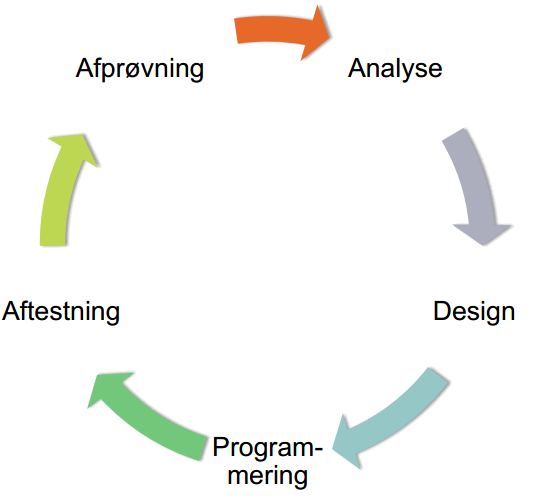
\includegraphics[scale=0.5]{billeder/evolutionaeremetode.png}
	\capt{Figuren illustrerer en fase i den evolutionære udviklingsmetode. En enkelt fase i udviklingsforløbet gennemgår samtlige dele af projektet.}
	\label{fig:evolutionaeremetode}
  \end{figure}

Modsat findes den konstruktive udviklingsmetode (også kaldet vandfaldsmetoden), som har en liniær tilgang til udviklingsprocessen. Den konstruktive udviklingsmetode er også delt op i faser, men hver fase er, modsat i den evolutionære metode, fokuseret henimod en specifik projektdel (se \figref{fig:konstruktivemetode}). Typisk vil et systemudviklingsforløb med udgangspunkt i den kontruktive udviklingsmetode starte ud med en analyse. Når analysen er færdig, påbegyndes design, og derefter programmering osv. Metoden bruges ofte i systemudviklingsprocesser, hvor det problem, der arbejdes ud fra, er veldefineret og klart. Det er grundet, at metoden ikke, på samme måde som den evolutionære udviklingsmetode, er dynamisk i forhold til, hvis problemet ændrer sig undervejs i forløbet.

\begin{figure}[ht]
	\centering
	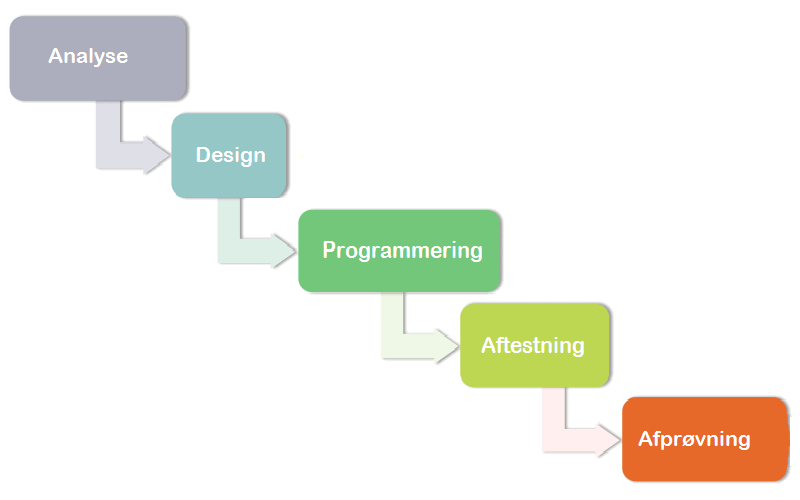
\includegraphics[scale=0.5]{billeder/konstruktivemetode.png}
  	\capt{Figuren illustrerer den konstruktive udviklingsmetode.}
  	\label{fig:konstruktivemetode}
\end{figure}

En forskel på de to metoder er bl.a. deres måde at interagere med brugere/informanter på. Mens der foregår et tæt samarbejde med informanter i den evolutionære udviklingsmetode, hvor der anvendes prototyper; har informanterne en mere passiv rolle i den konstruktive metode, hvor de blot godkender beslutninger, og fungerer som ressourcer til information. En anden forskel mellem de to metoder er deres tilgang til det endelig produkt/system. Den konstruktive udviklingsmetode har en meget stringent og langsigtet tidsplan, og man er ikke i tvivl om, hvornår produktet/systemet er færdigt. I en systemudviklingsproces med den evolutionære udviklingsmetode kan det modsat være svært at vurdere,  hvornår systemet er færdigt. Det vil altid være muligt at gå igennem endnu en iteration, og lave nye tilføjelser og redigeringer.

\begin{figure}[ht]
	\centering
	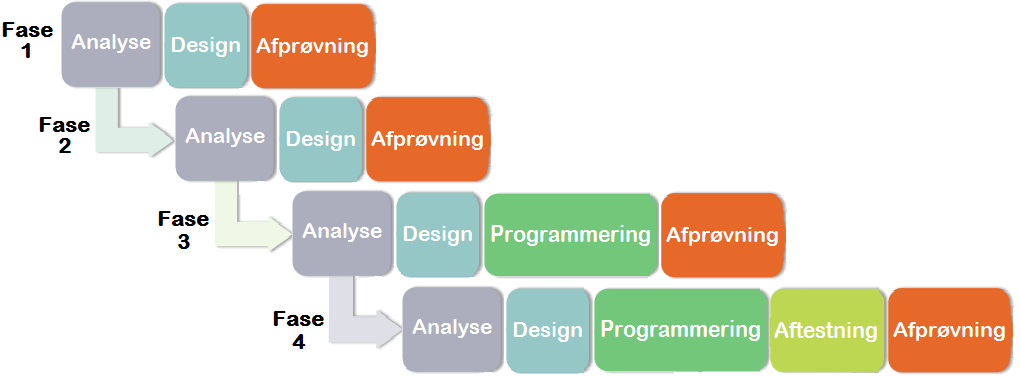
\includegraphics[scale=0.5]{billeder/blandingsmetode.png}
  	\capt{Figuren illustrerer gruppens udviklingsmetode, som har været en blanding mellem den evolutionære- og den konstruktive udviklingsmetode.}
  	\label{fig:blandingsmetode}
\end{figure}

Der er altså store forskelle på de to udviklingsmetoders tilgang til en systemudviklingsproces, og det er derfor op til situationen, hvilken der vil fungere bedst. Det er dog væsentligt at nævne, at det næsten aldrig vil være muligt udelukkende at arbejde ud fra den ene udviklingsmetode. Som regel vil elementer fra begge udviklingsmetoder blive implementeret. I vores projektforløb, anvendte vi også elementer fra begge metoder, men udgangspunktet var den evolutionære udviklingsmetode. Dette var grundet, at problemet som vi fokuserede på, ikke var fuldkommen klart i den initierende del af forløbet. Vi havde kurser, sideløbende med projektet, som gjorde, at vi ikke kunne komme igennem hver eneste projektdel, da vi først skulle introduceres for nogle begreber, i vores kurser omhandlende Systemudvikling \cite{ooad} og Designing Interactive Systems \cite{deb}. Vores udviklingsmetode er illustreret i \figref{fig:blandingsmetode}. Vi delte processen op i fire faser, hvor vi i de to første faser, udelukkende arbejdede med analyse, design og afprøvning ved hjælp af prototyper. Først i tredje fase begyndte vi at programmere og teste systemet, og det samme gjorde vi i fase fire. Den måde vores forløb var iterativt på, var ved at vi i hver fase gik tilbage, og tilføjede, redigerede eller slettede noget i de dele, som vi havde gennemgået i den foregående fase.

Til fremtidige projekter, ville den evolutionære udviklingsmetode bestemt være en metode gruppen ville overveje at bruge igen i lignende forløb. Den tætte interaktion med brugere/informanter, mener vi er essentiel i systemudvikling, fordi det i sidste ende er brugerne, som skal bruge det færdige system, og derfor er det vigtigt at systemet opfylder brugernes behov. Derudover er der det faktum, at metoden er så fleksibel som den er, hvilket gør den mere anvendelig til projektforløb end den konstruktive udviklingsmetode. Dette er grundet, at der sideløbende med projektet, ofte er kurser, som introducerer begreber, der skal implementeres til projektet, hvilket er nemmere med den evolutionære metode. Dette mener vi tilgengæld også er den evolutionære metodes største svaghed, da de konstante tilføjelser og redigeringer, også kræver en revidering af dokumentationen i form af rapporten. Det vil sige, at selv i et projektforløbs afsluttende fase, kan der stadig blive revideret i rapportens analysedel, designdel osv., og det giver en stor udfordring i forhold til at bibeholde en naturlig sammenhæng i rapporten, hvilket også er meget tidskrævende.

%% DONE:
%% Hvordan kunne det være blevet gjort bedre i fremtidige projekter?
%% konstruktive metode
%% fordele og ulember
%% Hvad har vi anvendt?
